\documentclass[10pt]{article}
\usepackage{amsmath}
\usepackage{geometry}
\usepackage{fancybox}
\usepackage{tikz}
\usepackage{listings}
 \geometry{
 a4paper,
 total={170mm,257mm},
 left=20mm,
 top=-5mm,
 }

\linespread{1.3}

\title{CSC263H1 Assignment 3}
\author{Jiatao Xiang, Xu Wang, Huakun Shen}
\date{February 14th, 2019}

\begin{document}
\maketitle

\section*{Question 1}
\textbf{Insert:}\\
\ovalbox{
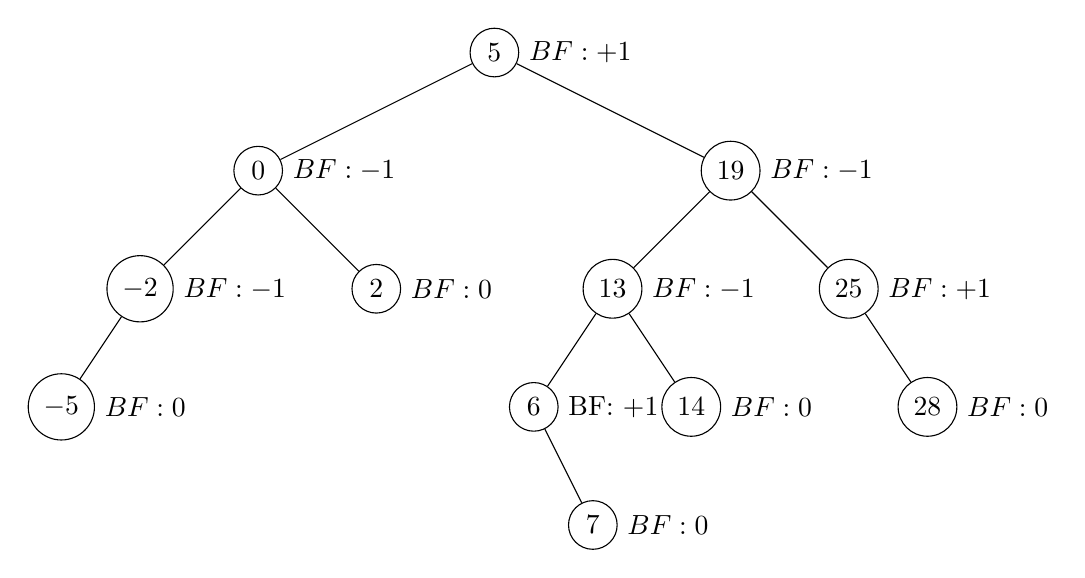
\begin{tikzpicture}[level/.style={sibling distance=60mm/#1}]
\node [circle,draw, label=right:$BF: +1$] (z){$5$}
  child {node [circle,draw, label=right:$BF: -1$] (lz) {$0$}
    child {node [circle,draw, label=right:$BF: -1$] (llz) {$-2$}
      child {node [circle, draw, label=right:$BF: 0$] (lllz) {$-5$}}
      child[fill=none]{edge from parent[draw=none]} 
    }
    child {node [circle,draw, label=right:$BF: 0$] (lrz) {$2$}
    }
  }
  child {node [circle,draw, label=right:$BF: -1$] (rz) {$19$}
    child {node [circle,draw, label=right:$BF: -1$] (rlz) {$13$}
    	child {node [circle, draw, label=right:BF: +1] (rllz) {$6$}
    		child[fill=none]{edge from parent[draw=none]}
    		child {node [circle, draw, label=right:$BF: 0$] (rllrz) {$7$}}
    	}
    	child {node [circle, draw, label=right:$BF: 0$] (rlrz) {$14$}}
    }
  child {node [circle,draw, label=right:$BF: +1$] (rrz) {$25$}
    child[fill=none]{edge from parent[draw=none]}
    child {node [circle, draw, label=right:$BF: 0$] (rrrz) {$28$}}		
	}
};
\end{tikzpicture}
}

\textbf{delete:}\\
\ovalbox{
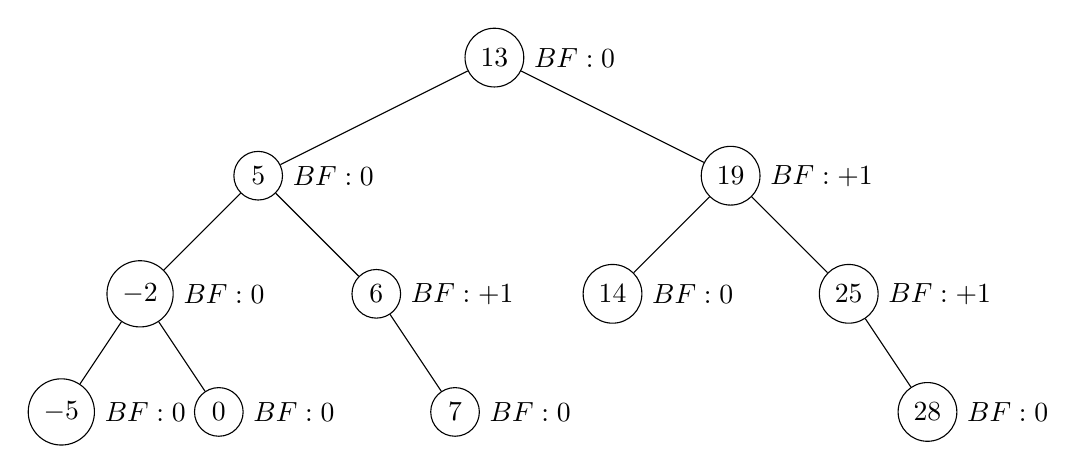
\begin{tikzpicture}[level/.style={sibling distance=60mm/#1}]
\node [circle,draw, label=right:$BF: 0$] (z){$13$}
  child {node [circle,draw, label=right:$BF: 0$] (lz) {$5$}
    child {node [circle,draw, label=right:$BF: 0$] (llz) {$-2$}
      child {node [circle, draw, label=right:$BF: 0$] (lllz) {$-5$}}
      child {node [circle, draw, label=right:$BF: 0$] (lllz) {$0$}}
    }
    child {node [circle,draw, label=right:$BF: +1$] (lrz) {$6$}
    	child[fill=none]{edge from parent[draw=none]}
    	child {node [circle, draw, label=right:$BF: 0$] (b) {$7$}}
    }
  }
  child {node [circle,draw, label=right:$BF: +1$] (rz) {$19$}
    child {node [circle,draw, label=right:$BF: 0$] (rlz) {$14$}
    }
  child {node [circle,draw, label=right:$BF: +1$] (rrz) {$25$}
    child[fill=none]{edge from parent[draw=none]}
    child {node [circle, draw, label=right:$BF: 0$] (rrrz) {$28$}}		
	}
};
\end{tikzpicture}
}
\section*{Question 2}


\section*{Question 3}


\end{document}
